\documentclass[11pt,letterpaper]{article}
\usepackage[lmargin=1in,rmargin=1in,bmargin=1in,tmargin=1in]{geometry}
\usepackage{style}

\setlength{\parindent}{0ex}

% -------------------
% Content
% -------------------
\begin{document}

% Title 
\begin{center} {\bfseries \Large MATH 122 \par\vspace{0.3cm} \LARGE Exam 2 Review} \end{center} \par

Exam 2 will be selected from the combinations of problems/parts of the graded and ungraded homeworks on WileyPlus. Problems may be slightly modified, i.e. values in the problem changed, the names or context changed, parts added or removed, plots changed, etc. The problems below represent a sample of what an exam resulting from this process could resemble. \pspace

% Problem 1
\prob Consider the function $f(x)$ plotted below. 
	\[
	\fbox{
	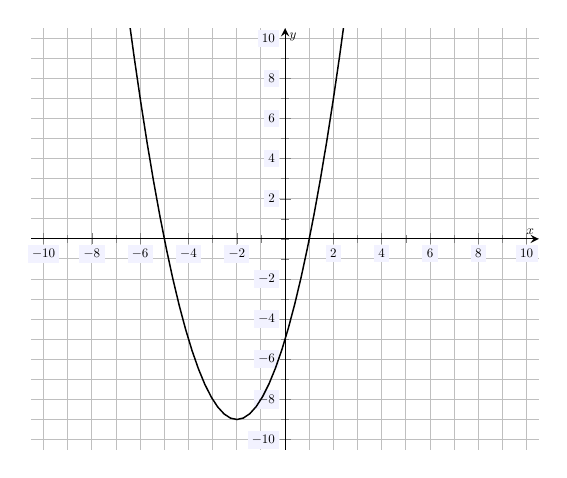
\begin{tikzpicture}[scale=0.94,every node/.style={scale=0.5}]
	\begin{axis}[
	grid=both,
	axis lines=middle,
	ticklabel style={fill=blue!5!white},
	xmin= -10.5, xmax=10.5,
	ymin= -10.5, ymax=10.5,
	xtick={-10,-8,-6,-4,-2,0,2,4,6,8,10},
	ytick={-10,-8,-6,-4,-2,0,2,4,6,8,10},
	minor tick = {-10,-9,...,10},
	xlabel=\(x\),ylabel=\(y\),
	]
	\addplot[line width= 0.02cm,samples=80,domain= -10.5:10.5] ({x},{(x - 1)*(x + 5)});
	\end{axis}
	\end{tikzpicture}
	}
	\] 

\begin{enumerate}[(a)]
\item When is $f'(x) > 0$? When is $f'(x) < 0$? Explain.
\item When is $f''(x) > 0$? When is $f''(x) < 0$? Explain. 
\item List any critical values for $f(x)$. Classify them as maxima or minima. 
\item Are there any points of inflection? Explain. 
\item Determine whether the following values are positive, negative, or zero:
	\begin{itemize}
	\item $f(-6)$
	\item $f'(1)$
	\item $f''(-3)$
	\item $f'(-2)$
	\end{itemize}
\item Sketch the tangent line to $f(x)$ at $x= -5$. 
\end{enumerate} 



% Problem 2
\prob Showing all your work, compute the following derivatives:
	\begin{enumerate}[(a)]
	\item $\dfrac{d}{dx} \, (5x^4 - 7x + 2 \sqrt[3]{x} - \pi^2)$
	\item $\dfrac{d}{dx} \left( 3x^4 \log_5 x \right)$
	\item $\dfrac{d}{dx} (e^x - 4)^8$
	\item $\dfrac{d}{dx} \left( \dfrac{5x - 1}{2x + 4} \right)$
	\end{enumerate}


% Problem 3
\prob Below is a plot of the derivative, $f'(x)$, of some function $f(x)$. Based on this plot, answer the questions below. 
	\[
	\fbox{
	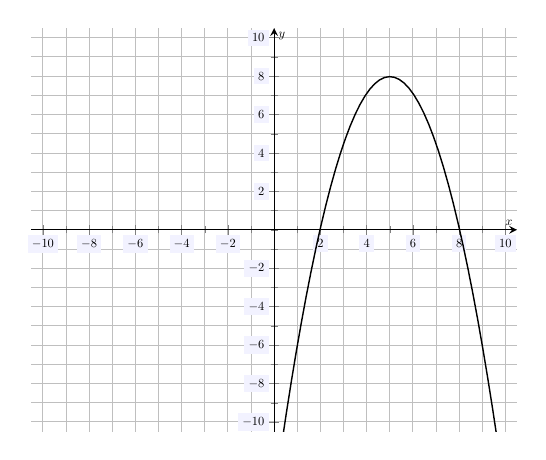
\begin{tikzpicture}[scale=0.9,every node/.style={scale=0.5}]
	\begin{axis}[
	grid=both,
	axis lines=middle,
	ticklabel style={fill=blue!5!white},
	xmin= -10.5, xmax=10.5,
	ymin= -10.5, ymax=10.5,
	xtick={-10,-8,-6,-4,-2,0,2,4,6,8,10},
	ytick={-10,-8,-6,-4,-2,0,2,4,6,8,10},
	minor tick = {-10,-9,...,10},
	xlabel=\(x\),ylabel=\(y\),
	]
	\addplot[line width= 0.02cm,samples=100,domain= -10.5:10.5] ({x},{-7/8*(x - 8)*(x - 2)+0.1});
	\end{axis}
	\end{tikzpicture}
	}
	\] 

\begin{enumerate}[(a)]
\item Where is $f(x)$ increasing? Where is $f(x)$ decreasing?
\item Find and classify any local maxima and minima for $f(x)$.
\item Where is $f(x)$ concave up? Where is $f(x)$ concave down?
\item Does $f(x)$ have any points of inflection? Explain. 
\end{enumerate} \pspace



% Problem 4
\prob Showing all your work, compute the following derivatives:
	\begin{enumerate}[(a)]
	\item $\dfrac{d}{dx} \left( x^6 4^{-x} \log_2(3x) \right)$
	\item $\dfrac{d}{dx} (x 9^{\sqrt{x}} - 5)^6$
	\item $\dfrac{d}{dx} \left( \dfrac{3^x \ln x}{5x - 4} \right)$
	\end{enumerate} \pspace



% Problem 5
\prob Suppose that the total cost, $C$, of producing $q$ items is given by $C(q)= 3q^2 + 150$. 
	\begin{enumerate}[(a)]
	\item Use the definition of the derivative to approximate $C'(2)$.
	\item What is the marginal cost when $q= 2$?
	\item Find the tangent line to $C(q)$ when $q= 2$.
	\item Use the previous part to estimate $C(2.2)$. 
	\item Knowing that $C''(2)= 6 > 0$, is your answer in (d) an overestimate or underestimate? 
	\end{enumerate} \pspace



% Problem 6
\prob Suppose that $f(x)= 2x^3 + 3x^2 - 120x$. 
	\begin{enumerate}[(a)]
	\item Where is $f(x)$ increasing? Where is $f(x)$ decreasing?
	\item Where is $f(x)$ concave up? Where is $f(x)$ concave down?
	\item Does $f(x)$ have any points of inflection?
	\item Find and classify any local maxima and local minima. 
	\item Find the global maxima and global minima for $f(x)$ on $[-2, 4]$.
	\end{enumerate}


\end{document}